% XCircuit output "schema_sim_L3ekvL4.tex" for LaTeX input from schema_sim_L3ekvL4.ps
\def\putbox#1#2#3#4{\makebox[0in][l]{\makebox[#1][l]{}\raisebox{\baselineskip}[0in][0in]{\raisebox{#2}[0in][0in]{\scalebox{#3}{#4}}}}}
\def\rightbox#1{\makebox[0in][r]{#1}}
\def\centbox#1{\makebox[0in]{#1}}
\def\topbox#1{\raisebox{-0.60\baselineskip}[0in][0in]{#1}}
\def\midbox#1{\raisebox{-0.20\baselineskip}[0in][0in]{#1}}
   \scalebox{0.8}{
   \normalsize
   \parbox{5.19792in}{
   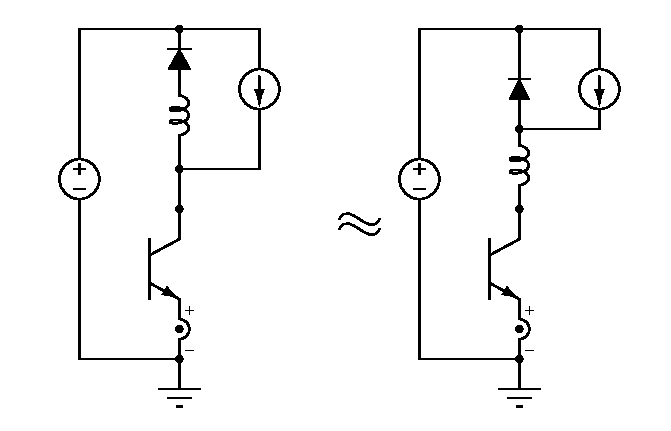
\includegraphics[scale=1.25]{schema_sim_L3ekvL4}\\
   % translate x=519 y=651 scale 0.30
   \putbox{1.48in}{2.44in}{1.20}{$L_{par}$}%
   \putbox{0.06in}{1.96in}{1.20}{$$}%
   \putbox{1.36in}{1.71in}{1.20}{\midbox{meraci bod}}%
   \putbox{4.31in}{2.02in}{1.20}{$L_{par}$}%
   \putbox{4.19in}{1.71in}{1.20}{\midbox{meraci bod}}%
   } % close 'parbox'
   } % close 'scalebox'
   \vspace{-\baselineskip} % this is not necessary, but looks better
